%!TEX root = ../../main.tex

\documentclass[../../main.tex]{subfiles}

\begin{document}
	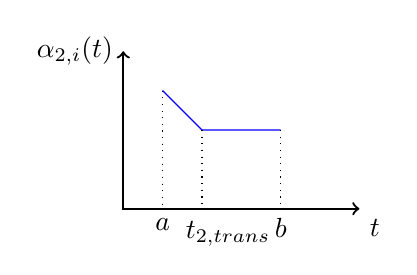
\begin{tikzpicture}[scale=1]
		\draw [thick,<->] (0,2) node [left] {$\alpha_{2,i}(t)$}--(0,0)--(3,0) node [below right] {$t$};
		\draw [blue] (0.5,1.5)--(1,1)--(2,1);
		\draw [dotted] (1,1)--(1,0) node [anchor=north west, pos=1.3, inner sep=-6pt] {$t_{2,\operatorname{trans}}$};
		\draw [dotted] (0.5,1.5)--(0.5,0) node [below] {$a$};
		\draw [dotted] (2,1)--(2,0) node [below] {$b$};
	\end{tikzpicture}
\end{document}